\documentclass[11pt]{article}

\usepackage[margin=1in]{geometry}
\usepackage{graphicx}
\usepackage{booktabs}
\usepackage{array}
\usepackage{hyperref}
\usepackage{xcolor}
\usepackage{amsmath}
\usepackage{microtype}

\hypersetup{
  colorlinks=true,
  linkcolor=blue!45!black,
  citecolor=blue!45!black,
  urlcolor=blue!45!black
}

\newcommand{\model}[1]{\textsc{#1}}

\title{Evaluating Frontier Language Models on Clinician-Reviewed Dental Questions: A Reproducible Benchmark}

\author{
Francisco Teixeira Barbosa\\
Foundation for Oral Rehabilitation\\
\texttt{francisco@for.org}
\and
Daniel Robles Cantero\\
Universidad Europea Miguel de Cervantes\\
\texttt{drobles@clinica.uemc.es}
\and
Aritza Brizuela Velasco\\
Universidad Europea Miguel de Cervantes\\
\texttt{abrizuela@uemc.es}
}

\date{Draft of June 11, 2026}

\begin{document}

\maketitle

\begin{abstract}
Large language models (LLMs) are increasingly used to answer clinical questions, but general medical benchmarks do not directly test whether models can answer guideline-grounded dental questions that occur in periodontology, implant dentistry, oral-systemic medicine, pharmacology, and patient communication.
We present a clinician-reviewed dental question-answering benchmark containing 30 open-ended questions across six clinical domains, each paired with explicit \emph{must include} and \emph{must avoid} rubric criteria.
We evaluated eight contemporary LLMs available through OpenRouter on June 10--11, 2026, using single-trial, temperature-0 prompting and a rubric-based LLM judge.
The leading deployment accuracies were GPT-5.2 at 96.7\%, Claude Opus 4.8 and GPT-5.5 at 93.3\%, and Gemini 3.1 Pro at 90.0\%, but bootstrap confidence intervals over questions were wide and overlapped substantially.
Claude Fable 5 answered only 25 of 30 questions because of refusals concentrated in oral-systemic topics; on answered questions it reached 96.0\% accuracy.
Two additional OpenAI-family judges showed only moderate agreement with the primary Claude Opus 4.8 judge (81.7--83.8\% verdict agreement; Cohen's $\kappa=0.506$--0.524), emphasizing that absolute accuracy levels are judge-dependent.
The benchmark, transcripts, rubrics, and analysis code are released to support reproducible, specialty-specific evaluation of LLMs in dentistry.
\end{abstract}

\section{Introduction}

Medical question answering has become a central test case for large language models.
MultiMedQA and Med-PaLM showed that LLMs can encode substantial clinical knowledge while also exposing gaps in factuality, reasoning, potential harm, and bias that matter for clinical deployment \cite{singhal2023clinical}.
HealthBench extended open-ended health evaluation through physician-written rubric criteria, underscoring the value of explicit scoring rubrics over answer-only multiple-choice accuracy \cite{arora2025healthbench}.
Biomedical QA benchmarks such as PubMedQA provide useful tests of biomedical reasoning over abstracts \cite{jin2019pubmedqa}, but dentistry-specific clinical questions remain underrepresented in widely used benchmarks.

Dentistry is not a narrow variant of general medicine for evaluation purposes.
Clinically useful dental answers often depend on specialty-specific consensus frameworks and guidelines, including the 2017 World Workshop classification of periodontal and peri-implant diseases \cite{tonetti2018staging,papapanou2018periodontitis}, the EFP S3 treatment guideline for stages I--III periodontitis \cite{sanz2020efp}, AAOMS guidance on medication-related osteonecrosis of the jaw \cite{ruggiero2022mronj}, and current infective-endocarditis prophylaxis statements \cite{wilson2021ie}.
Small omissions can change clinical meaning: for example, failing to distinguish periodontal stability endpoints from treatment thresholds, or giving jurisdiction-insensitive antibiotic prophylaxis advice, may produce a fluent but unsafe answer.

Recent dental LLM studies have evaluated models on dental multiple-choice questions \cite{nguyen2025dentalmcq}, implantology scenarios \cite{wu2025implantology}, and open-ended periodontology examination answers \cite{ramlogan2025periodontology}.
Broader dental benchmark efforts include DentalBench \cite{zhu2025dentalbench} and the concurrent GlobalDentBench \cite{zhao2026globaldentbench}.
GlobalDentBench is substantially larger and multinational, whereas the present work contributes a smaller but fully public, auditable benchmark focused on clinically realistic, guideline-grounded dental questions with explicit scoring rubrics, answer transcripts, judge verdicts, and cross-judge agreement analysis.

\section{Methods}

\subsection{Benchmark Dataset}

The benchmark contains 30 open-ended questions across six domains: periodontal diagnosis, periodontal treatment, implants and peri-implantitis, oral-systemic medicine, pharmacology, and patient communication.
Each domain contributes five questions.
Question difficulty labels were assigned as basic (7 questions), intermediate (14 questions), or advanced (9 questions).
Each question includes a rubric specifying required concepts and prohibited errors.
An answer is scored correct only if it satisfies all required criteria and commits no prohibited error.

The rubrics were authored and reviewed by a periodontist and checked against guideline sources before the reported run.
The validation log records verification against primary or authoritative sources for the highest-risk factual claims, including periodontal staging and grading, EFP treatment endpoints, diabetes-periodontitis effect sizes, MRONJ drug classes, infective endocarditis prophylaxis, and anticoagulant management.
No patient records, radiographs, or protected health information were used.

\subsection{Models and Execution}

We evaluated eight models through the OpenRouter chat-completions API on June 10--11, 2026.
The model roster is shown in Table~\ref{tab:models}.
All candidate-answer calls used temperature 0 and a maximum completion budget of 12,000 tokens.
Each model answered each question once.
The run therefore produced 240 model-question rows.
Latency was measured as wall-clock time for each candidate-answer request.

\begin{table}[t]
\centering
\caption{Model roster evaluated in the reported run. Model identifiers are the OpenRouter identifiers recorded by the benchmark harness.}
\label{tab:models}
\begin{tabular}{lll}
\toprule
Label & OpenRouter model identifier & Tier \\
\midrule
Claude Fable 5 & \texttt{anthropic/claude-fable-5} & Flagship \\
Claude Opus 4.8 & \texttt{anthropic/claude-opus-4.8} & Flagship \\
GPT-5.5 & \texttt{openai/gpt-5.5} & Flagship \\
GPT-5.2 & \texttt{openai/gpt-5.2} & Flagship \\
Gemini 3.1 Pro & \texttt{google/gemini-3.1-pro-preview} & Flagship \\
Qwen3.7 Plus & \texttt{qwen/qwen3.7-plus} & Efficient \\
Llama 4 Maverick & \texttt{meta-llama/llama-4-maverick} & Open-weight \\
DeepSeek V3.2 & \texttt{deepseek/deepseek-v3.2} & Open-weight \\
\bottomrule
\end{tabular}
\end{table}

\subsection{Rubric-Based Judging}

The primary judge was Claude Opus 4.8, queried through the same OpenRouter client.
The judge received the clinical question, the question-specific rubric, and the candidate answer, and returned a structured JSON verdict containing the number of required criteria satisfied, the total number of required criteria, any prohibited violations, a Boolean correctness verdict, and a brief explanation.
This LLM-as-judge design follows the general direction of scalable model-assisted evaluation \cite{zheng2023judge} and health-domain rubric evaluation \cite{arora2025healthbench}, but we treated judge dependence as an empirical quantity rather than an assumption.

To measure judge dependence, all non-empty stored answers were independently re-scored with GPT-5.2 and GPT-5.5 as secondary judges.
This check was motivated by reported self-recognition and self-preference biases in LLM-based evaluation \cite{panickssery2024selfrecognition,wataoka2024selfpreference}.
Because Claude Fable 5 refused five questions and produced no answer text for those rows, the paired judge-agreement analyses included 235 answered rows.
We report raw verdict agreement and Cohen's kappa for each secondary judge pass.

\subsection{Outcomes}

The primary outcome was deployment accuracy: the proportion of all 30 questions scored correct for a model, counting refusals and empty answers as incorrect.
We also report answer rate, accuracy among answered rows, and mean latency.
For per-model uncertainty, we computed bootstrap 95\% intervals over questions using 10,000 resamples in \texttt{src/analysis.py}, resetting Python's \texttt{random.Random(42)} per model.
These intervals reflect the small question set and should not be interpreted as formal population-level confidence intervals over all possible dental questions.

\section{Results}

\subsection{Overall Accuracy}

Across all 240 model-question rows, primary-judge accuracy was 81.7\%.
Table~\ref{tab:results} summarizes per-model accuracy, answer rate, accuracy on answered rows, and mean latency.
GPT-5.2 achieved the highest deployment accuracy at 96.7\% (29/30), followed by Claude Opus 4.8 and GPT-5.5 at 93.3\% (28/30), Gemini 3.1 Pro at 90.0\% (27/30), Qwen3.7 Plus at 83.3\% (25/30), Claude Fable 5 at 80.0\% (24/30), DeepSeek V3.2 at 70.0\% (21/30), and Llama 4 Maverick at 46.7\% (14/30).

\begin{table}[t]
\centering
\caption{Primary benchmark results. Accuracy counts refusals as incorrect. Confidence intervals are bootstrap intervals over 30 questions.}
\label{tab:results}
\begin{tabular}{lrrrr}
\toprule
Model & Accuracy (95\% CI) & Answer rate & Accuracy on answered & Mean latency \\
\midrule
GPT-5.2 & 96.7\% [90.0, 100] & 100\% & 96.7\% & 14.8 s \\
Claude Opus 4.8 & 93.3\% [83.3, 100] & 100\% & 93.3\% & 12.1 s \\
GPT-5.5 & 93.3\% [83.3, 100] & 100\% & 93.3\% & 20.1 s \\
Gemini 3.1 Pro & 90.0\% [76.7, 100] & 100\% & 90.0\% & 20.5 s \\
Qwen3.7 Plus & 83.3\% [70.0, 96.7] & 100\% & 83.3\% & 40.8 s \\
Claude Fable 5 & 80.0\% [66.7, 93.3] & 83.3\% & 96.0\% & 16.5 s \\
DeepSeek V3.2 & 70.0\% [53.3, 86.7] & 100\% & 70.0\% & 34.1 s \\
Llama 4 Maverick & 46.7\% [30.0, 63.3] & 100\% & 46.7\% & 25.7 s \\
\bottomrule
\end{tabular}
\end{table}

Figure~\ref{fig:accuracy-model} shows the same ranking with bootstrap intervals.
The top four models have heavily overlapping intervals, and this study should not be cited as evidence of a statistically resolved ordering among those frontier systems.
The larger separation between the leading cluster and the open-weight models was more pronounced.

\begin{figure}[t]
\centering
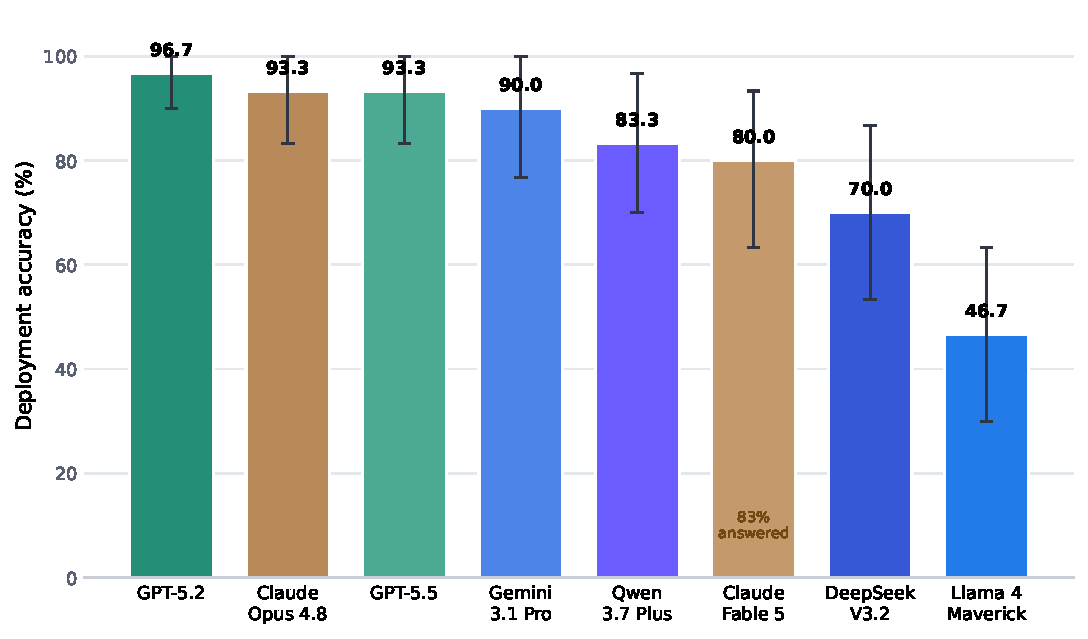
\includegraphics[width=\linewidth]{figures/accuracy_by_model_arxiv.pdf}
\caption{Deployment accuracy by model. Error bars show bootstrap 95\% intervals over questions. Refusals are counted as incorrect.}
\label{fig:accuracy-model}
\end{figure}

\subsection{Domain Patterns}

Figure~\ref{fig:accuracy-domain} shows accuracy by clinical domain.
Pharmacology was the clearest differentiator: Llama 4 Maverick scored 0\% in this domain, while GPT-5.2, GPT-5.5, Claude Opus 4.8, Claude Fable 5, and DeepSeek V3.2 performed better.
DeepSeek V3.2 was weakest in periodontal diagnosis and treatment.
Qwen3.7 Plus showed strong performance for an efficient-tier model, with 83.3\% deployment accuracy overall.

\begin{figure}[t]
\centering
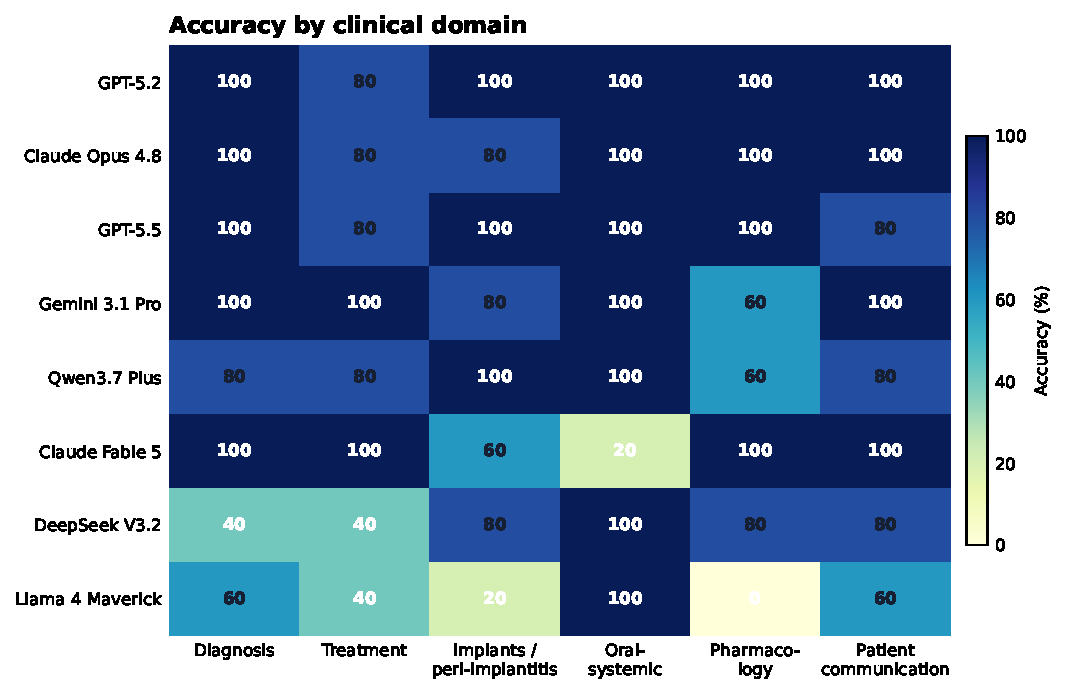
\includegraphics[width=\linewidth]{figures/accuracy_by_domain_arxiv.pdf}
\caption{Accuracy by model and clinical domain. Each cell contains five questions.}
\label{fig:accuracy-domain}
\end{figure}

\subsection{Refusals and Empty Answers}

Claude Fable 5 refused five of 30 questions.
The refused topics clustered in oral-systemic evidence and peri-implant soft-tissue topics: diabetes and periodontitis, pregnancy and periodontal treatment, smoking and periodontitis, periodontitis and Alzheimer's disease, and supracrestal tissue attachment around implants.
This produced an 83.3\% answer rate and an 80.0\% deployment accuracy, despite 96.0\% accuracy among answered questions.
Repository serving notes indicate that the same refusal behavior reproduced across both Amazon Bedrock and Anthropic first-party serving.
For clinical deployment, this distinction matters: a model that refuses clinically relevant questions may be safer than one that hallucinates, but it is not equivalent to a system that gives a correct, calibrated answer.

\subsection{Judge Agreement}

The GPT-5.2 secondary judge agreed with the Claude Opus 4.8 primary judge on 81.7\% of paired answered rows, with Cohen's $\kappa=0.506$.
The GPT-5.5 secondary judge agreed on 83.8\% of paired answered rows, with $\kappa=0.524$.
Both OpenAI judges were stricter than the primary judge overall.
For example, GPT-5.5 scored its own GPT-5.5 answers at 76.7\%, whereas the Claude Opus 4.8 primary judge scored the same GPT-5.5 answers at 93.3\%.
This pattern argues against a simple same-family favoritism explanation and reinforces that absolute accuracy should be interpreted as judge-dependent.

\section{Discussion}

This benchmark suggests that contemporary frontier LLMs can answer many guideline-grounded dental questions, but it also shows why specialty-specific evaluation remains necessary.
The highest-scoring systems performed well on the small question set, yet their confidence intervals overlap, their errors occur in clinically meaningful places, and the judge-agreement analysis shows only moderate inter-judge reliability.
Ranking frontier models from a 30-question benchmark would therefore be overconfident.
The more defensible conclusion is that a leading cluster performed substantially better than weaker open-weight systems on this particular dental task set, while refusal behavior and domain-specific failure modes changed the deployment interpretation.

Open-ended dental QA differs from multiple-choice dental examinations.
Multiple-choice benchmarks are easier to scale and compare, but they can hide clinically important omissions.
In this benchmark, a candidate answer can be fluent and plausible yet still fail if it omits a required action threshold, fails to mention irreversibility of established bone loss in patient communication, or presents a jurisdiction-specific prophylaxis guideline as universal.
The rubric-based design is intended to expose those omissions.

At the same time, the method remains preliminary.
The question set is small, the rubrics were reviewed by one periodontist, only one candidate-answer trial was used, and LLM-as-judge scoring is not a substitute for independent human adjudication.
The secondary-judge passes quantify this problem rather than solve it.
Future versions should expand the dataset, include multiple calibrated dental experts, use repeated trials, adjudicate disagreement rows manually, and separate knowledge recall, clinical reasoning, patient communication, and potential-harm scoring.

\section{Limitations}

First, the benchmark contains only 30 questions, with five per domain.
The bootstrap intervals are consequently wide, and small accuracy differences should be treated as noise.
Second, the final eight-model run used a single trial at temperature 0.
Earlier five-model end-to-end runs showed at most a one-question per-model shift, but full eight-model run-to-run stability was not measured.
Third, the primary ground truth is a single-clinician, guideline-checked rubric set rather than a multi-expert consensus panel.
Fourth, all primary verdicts rely on an LLM judge, and secondary judges showed only moderate agreement with the primary judge.
Fifth, the results reflect model availability, model versions, and OpenRouter routing on June 10--11, 2026.
Model identifiers and behavior may drift.
Finally, the benchmark evaluates text answers to simulated questions; it does not validate clinical deployment, patient outcomes, chairside decision support, or regulatory safety.

\section{Data and Code Availability}

The benchmark code, dataset, raw JSONL results, transcripts, judge verdicts, plotting scripts, and reproducible analysis script are available at:
\begin{center}
\url{https://github.com/Tuminha/llm-evaluation-for-dentistry}
\end{center}
The repository commit containing the reported 240-row primary results file, both 235-row secondary judge files, and \texttt{src/analysis.py} is:
\begin{center}
\texttt{416104585625b211732bd7355636fda8d625075f}
\end{center}

\section{Ethics Statement}

This study used clinician-authored benchmark questions and guideline-derived rubrics.
It did not use patient records, radiographs, clinical images, or protected health information.
The results should not be interpreted as validating any model for autonomous diagnosis, prescribing, treatment planning, or patient-specific clinical decision-making.

\section{Author Contributions}

Francisco Teixeira Barbosa designed the benchmark, implemented the evaluation harness, ran the analyses, and drafted the manuscript.
Daniel Robles Cantero and Aritza Brizuela Velasco contributed clinical and scientific review and manuscript-development support.

\section{Acknowledgments}

The authors acknowledge the Foundation for Oral Rehabilitation for support during preparation of this benchmark and manuscript.

\begin{thebibliography}{99}
\raggedright

\bibitem{singhal2023clinical}
K.~Singhal, S.~Azizi, T.~Tu, S.~S. Mahdavi, J.~Wei, H.~W. Chung, N.~Scales, A.~Tanwani, H.~Cole-Lewis, S.~Pfohl, et~al.
\newblock Large language models encode clinical knowledge.
\newblock \emph{Nature}, 620:172--180, 2023.
\newblock doi:10.1038/s41586-023-06291-2.

\bibitem{arora2025healthbench}
R.~K. Arora, J.~Wei, R.~S. Hicks, P.~Bowman, J.~Quinonero-Candela, F.~Tsimpourlas, M.~Sharman, M.~Shah, A.~Vallone, A.~Beutel, J.~Heidecke, and K.~Singhal.
\newblock HealthBench: Evaluating large language models towards improved human health.
\newblock arXiv:2505.08775, 2025.

\bibitem{jin2019pubmedqa}
Q.~Jin, B.~Dhingra, Z.~Liu, W.~Cohen, and X.~Lu.
\newblock PubMedQA: A dataset for biomedical research question answering.
\newblock In \emph{Proceedings of EMNLP-IJCNLP}, pages 2567--2577, 2019.
\newblock doi:10.18653/v1/D19-1259.

\bibitem{tonetti2018staging}
M.~S. Tonetti, H.~Greenwell, and K.~S. Kornman.
\newblock Staging and grading of periodontitis: Framework and proposal of a new classification and case definition.
\newblock \emph{Journal of Periodontology}, 89(Suppl 1):S159--S172, 2018.
\newblock doi:10.1002/JPER.18-0006.

\bibitem{papapanou2018periodontitis}
P.~N. Papapanou, M.~Sanz, N.~Buduneli, T.~Dietrich, M.~Feres, D.~H. Fine, T.~F. Flemmig, R.~Garcia, W.~V. Giannobile, F.~Graziani, et~al.
\newblock Periodontitis: Consensus report of workgroup 2 of the 2017 World Workshop on the Classification of Periodontal and Peri-Implant Diseases and Conditions.
\newblock \emph{Journal of Clinical Periodontology}, 45(Suppl 20):S162--S170, 2018.
\newblock doi:10.1111/jcpe.12946.

\bibitem{sanz2020efp}
M.~Sanz, D.~Herrera, M.~Kebschull, I.~Chapple, S.~Jepsen, T.~Berglundh, A.~Sculean, M.~Tonetti, and EFP Workshop Participants.
\newblock Treatment of stage I--III periodontitis: The EFP S3 level clinical practice guideline.
\newblock \emph{Journal of Clinical Periodontology}, 47(Suppl 22):4--60, 2020.
\newblock doi:10.1111/jcpe.13290.

\bibitem{ruggiero2022mronj}
S.~L. Ruggiero, T.~B. Dodson, T.~Aghaloo, R.~Carlson, B.~B. Ward, and D.~Kademani.
\newblock American Association of Oral and Maxillofacial Surgeons' position paper on medication-related osteonecrosis of the jaws--2022 update.
\newblock \emph{Journal of Oral and Maxillofacial Surgery}, 80(5):920--943, 2022.
\newblock doi:10.1016/j.joms.2022.02.008.

\bibitem{wilson2021ie}
W.~R. Wilson, M.~Gewitz, P.~B. Lockhart, A.~F. Bolger, D.~C. DeSimone, D.~S. Kazi, D.~J. Couper, A.~Beaton, C.~Kilmartin, J.~M. Miro, et~al.
\newblock Prevention of viridans group streptococcal infective endocarditis: A scientific statement from the American Heart Association.
\newblock \emph{Circulation}, 143(20):e963--e978, 2021.
\newblock doi:10.1161/CIR.0000000000000969.

\bibitem{nguyen2025dentalmcq}
H.~C. Nguyen, H.~P. Dang, T.~L. Nguyen, V.~Hoang, and V.~A. Nguyen.
\newblock Accuracy of latest large language models in answering multiple choice questions in dentistry: A comparative study.
\newblock \emph{PLOS ONE}, 20(1):e0317423, 2025.
\newblock doi:10.1371/journal.pone.0317423.

\bibitem{wu2025implantology}
X.~Wu, G.~Cai, B.~Guo, L.~Ma, S.~Shao, J.~Yu, Y.~Zheng, L.~Wang, and F.~Yang.
\newblock A multi-dimensional performance evaluation of large language models in dental implantology: Comparison of ChatGPT, DeepSeek, Grok, Gemini and Qwen across diverse clinical scenarios.
\newblock \emph{BMC Oral Health}, 25:1272, 2025.
\newblock doi:10.1186/s12903-025-06619-6.

\bibitem{ramlogan2025periodontology}
S.~Ramlogan, V.~Raman, and S.~Ramlogan.
\newblock A pilot study of the performance of Chat GPT and other large language models on a written final year periodontology exam.
\newblock \emph{BMC Medical Education}, 25:727, 2025.
\newblock doi:10.1186/s12909-025-07195-7.

\bibitem{zhu2025dentalbench}
H.~Zhu, Y.~Xu, Y.~Li, Z.~Meng, and Z.~Liu.
\newblock DentalBench: Benchmarking and advancing LLMs capability for bilingual dentistry understanding.
\newblock arXiv:2508.20416, 2025.

\bibitem{zhao2026globaldentbench}
J.~Zhao, J.~Liang, Z.~Cai, J.~Zhang, Z.~Wen, S.~Deng, W.~Yi, C.~Luo, H.~Zhang, J.~Chen, et~al.
\newblock GlobalDentBench: A multinational benchmark for evaluating LLM clinical reasoning in dentistry with expert calibration.
\newblock arXiv:2605.24636, 2026.

\bibitem{zheng2023judge}
L.~Zheng, W.-L. Chiang, Y.~Sheng, S.~Zhuang, Z.~Wu, Y.~Zhuang, Z.~Lin, Z.~Li, D.~Li, E.~P. Xing, et~al.
\newblock Judging LLM-as-a-judge with MT-Bench and Chatbot Arena.
\newblock In \emph{NeurIPS 2023 Datasets and Benchmarks Track}, 2023.
\newblock arXiv:2306.05685.

\bibitem{panickssery2024selfrecognition}
A.~Panickssery, S.~R. Bowman, and S.~Feng.
\newblock LLM evaluators recognize and favor their own generations.
\newblock arXiv:2404.13076, 2024.

\bibitem{wataoka2024selfpreference}
K.~Wataoka, T.~Takahashi, and R.~Ri.
\newblock Self-preference bias in LLM-as-a-judge.
\newblock arXiv:2410.21819, 2024.

\end{thebibliography}

\end{document}
